\section{CONVEX FUNCTIONS OF A REAL VARIABLE}

Let H be a subset of R, f a finite real function defined on H, and let G be the graph or representative set of the function f in \(R \times R = R^{2}\) , the set of points \(M_{x} = (x, f(x))\) , where x runs through H. It is convenient to say that a point \((a, b)\) of \(R^{2}\) such that \(a \in H\) lies above (resp. strictly above, below, strictly below) G if one has \(b \geqslant f(a)\) (resp. \(b > f(a), b \leqslant f(a), b < f(a)\) ). If \(A = (a, a')\) and \(B = (b, b')\) are two points of \(R^{2}\) we denote by AB the closed segment with endpoints A and B; if a \textless{} b then AB is the graph of the linear function \(a' + \frac{b' - a'}{b - a} (x - a)\) defined on {[}a, b{]}; we denote the slope \(\frac{b' - a'}{b - a}\) of this segment by \(p(\text{AB})\) , and will make use of the following lemma, whose verification is immediate:

Lemma. Let \(\mathrm{A} = (a, a')\) , \(\mathrm{B} = (b, b')\) , \(\mathrm{C} = (c, c')\) be three points in \(\mathbf{R}^2\) such that \(a < b < c\) . The following statements are equivalent:

\begin{enumerate}
\def\labelenumi{\alph{enumi})}
\item
  B is below AC;
\item
  C lies above the line passing through A and B;
\item
  A is above the line passing through B and C;
\item
  \(p(\mathrm{AB}) \leqslant p(\mathrm{AC});\)
\item
  \(p(\mathrm{AC}) \leqslant p(\mathrm{BC})\) .
\end{enumerate}

The lemma still holds when one replaces ``above'' (resp. ``below'') by ``strictly above'' (resp. ``strictly below'') and the sign \(\leqslant\) by \textless{} (fig.~1).

\pandocbounded{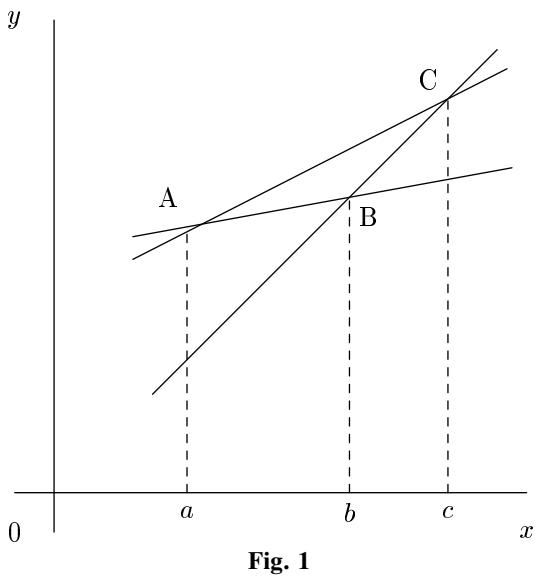
\includegraphics[keepaspectratio]{images/part001_7b60909a.jpg}}

